% example-1-damages.tex
% Self-contained extract from example.tex (compile: pdflatex example-1-damages.tex, run twice).

\documentclass[11pt]{article}

\usepackage[margin=1in]{geometry}
\usepackage{amsmath}
\usepackage{enumitem}
\usepackage{xcolor}
\usepackage{soul}
\usepackage{tikz}
\usetikzlibrary{arrows.meta,positioning,calc,backgrounds}

% --- atomic-unit highlight colours (one per cluster; F9 is the pivot) ---
\definecolor{cBreach}{RGB}{210,228,248}   % breach cluster (F1--F4)
\definecolor{cArgue} {RGB}{252,243,207}    % defendant's argument (F5--F6)
\definecolor{cAgree} {RGB}{215,236,219}    % agreement / fraud (F7,F8,F10)
\definecolor{cPivot} {RGB}{250,219,180}    % F9 void ab initio (pivot)
\definecolor{cUnjust}{RGB}{198,231,201}    % unjust enrichment (F11--F13)

% \fu{colour}{span}{label}: highlight a clause and tag it with its atomic-unit id.
% \hl (soul) wraps across line breaks; money amounts are kept in \mbox so the
% \$ does not trip soul's tokenizer.
\sethlcolor{cBreach}
\newcommand{\fu}[3]{{\sethlcolor{#1}\hl{#2}}\,\textsuperscript{\textbf{\scriptsize #3}}}

\title{Example 1: A Legal Damages Paragraph}
\author{FactReasoner --- Ideation}
\date{\today}

\begin{document}
\maketitle
\section{Source paragraph}

\noindent\textbf{Plain text.}
\begin{quote}
The defendant was found liable for breach of contract, which occurred on
March 15, 2022, after they failed to deliver the specified goods. As a result,
the court awarded the plaintiff \$50,000 in damages for the breach. However, the
defendant argued that the plaintiff's own actions constituted a prior breach,
thus excusing their performance. The case hinged on the initial agreement signed
on January 1, 2022, which the court ultimately declared void ab initio (void from
the beginning) due to fraudulent misrepresentation by the plaintiff. Separately,
the court found the defendant liable for unjust enrichment and awarded the
plaintiff \$10,000 on that basis, as the defendant had retained a down payment.
\end{quote}

\noindent\textbf{Annotated.} Each highlighted clause is one atomic unit, tagged
with its identifier \textsuperscript{\textbf{\scriptsize F\textit{n}}}. Colours
group the units into the four clusters used later in the relation graph.

\begin{quote}
The defendant was \fu{cBreach}{found liable for breach of contract}{F1}, which
occurred \fu{cBreach}{on March 15, 2022}{F2}, after they
\fu{cBreach}{failed to deliver the specified goods}{F3}. As a result, the court
\fu{cBreach}{awarded the plaintiff \mbox{\$50,000} in damages for the breach}{F4}.
However, the defendant argued that
\fu{cArgue}{the plaintiff's own actions constituted a prior breach}{F5},
\fu{cArgue}{thus excusing their performance}{F6}.
\fu{cAgree}{The case hinged on the initial agreement}{F7}, signed
\fu{cAgree}{on January 1, 2022}{F8}, which the court ultimately
\fu{cPivot}{declared void ab initio (void from the beginning)}{F9} due to
\fu{cAgree}{fraudulent misrepresentation by the plaintiff}{F10}. Separately, the
court \fu{cUnjust}{found the defendant liable for unjust enrichment}{F11} and
\fu{cUnjust}{awarded the plaintiff \mbox{\$10,000} on that basis}{F12}, as the
\fu{cUnjust}{defendant had retained a down payment}{F13}.
\end{quote}

\noindent{\footnotesize\textbf{Legend:}~
\sethlcolor{cBreach}\hl{~breach of contract (F1--F4)~}\quad
\sethlcolor{cArgue}\hl{~defendant's argument (F5--F6)~}\quad
\sethlcolor{cPivot}\hl{~pivot: void ab initio (F9)~}\\[2pt]
\sethlcolor{cAgree}\hl{~agreement / fraud (F7, F8, F10)~}\quad
\sethlcolor{cUnjust}\hl{~unjust enrichment (F11--F13)~}\quad
The tag \textsuperscript{\textbf{\scriptsize F\textit{n}}} gives each unit's id.}

\section{Atomic units (in order of appearance)}

An \emph{atomic unit} is a short, self-contained sentence carrying exactly one
fact or claim.

\begin{enumerate}[label=\textbf{F\arabic*.},leftmargin=*]
  \item The defendant was found liable for breach of contract.
  \item The breach of contract occurred on March 15, 2022.
  \item The defendant failed to deliver the specified goods.
  \item The court awarded the plaintiff \$50,000 in damages for the breach.
  \item The defendant argued that the plaintiff's own actions constituted a prior breach.
  \item The defendant argued that the plaintiff's prior breach excused the defendant's performance.
  \item The case hinged on the initial agreement.
  \item The initial agreement was signed on January 1, 2022.
  \item The court declared the initial agreement void ab initio (void from the beginning).
  \item The agreement was declared void due to fraudulent misrepresentation by the plaintiff.
  \item The court found the defendant liable for unjust enrichment.
  \item The court awarded the plaintiff \$10,000 on the basis of unjust enrichment.
  \item The defendant had retained a down payment.
\end{enumerate}

\section{Relations}

\subsection*{Logical prerequisites ($A \rightarrow B$)}
\begin{itemize}[leftmargin=*]
  \item F3 $\rightarrow$ F1 --- failing to deliver the goods grounds the breach finding.
  \item F1 $\rightarrow$ F2 --- the breach must exist for it to have a date.
  \item F1 $\rightarrow$ F4 --- liability for breach is required to award damages ``for the breach.''
  \item F7 $\rightarrow$ F1 --- an initial agreement must exist for there to be a contract to breach.
  \item F7 $\rightarrow$ F8 --- the agreement must exist for it to have a signing date.
  \item F7 $\rightarrow$ F9 --- the agreement must exist for the court to declare it void.
  \item F8 $\rightarrow$ F9 --- the agreement signed Jan~1, 2022 is the thing declared void.
  \item F10 $\rightarrow$ F9 --- fraudulent misrepresentation is the stated cause of the voidness.
  \item F13 $\rightarrow$ F11 --- retaining the down payment grounds the unjust-enrichment finding.
  \item F11 $\rightarrow$ F12 --- the unjust-enrichment finding grounds the \$10,000 award.
\end{itemize}

\subsection*{Position invalidations ($A \neq B$)}
\begin{itemize}[leftmargin=*]
  \item F9 $\neq$ F1 --- void \emph{ab initio} means no valid contract ever existed,
        so the earlier breach-of-contract finding is invalidated.
  \item F9 $\neq$ F2 --- a breach ``on March 15, 2022'' cannot stand once no valid
        contract existed on that date.
  \item F9 $\neq$ F4 --- the \$50,000 damages award rests on a breach that is now
        deemed never to have occurred.
  \item F9 $\neq$ F6 --- there was no valid performance obligation to be ``excused.''
  \item F10 $\neq$ F5 --- the plaintiff's fraud supersedes the defendant's
        ``prior breach by plaintiff'' argument with a stronger ground.
\end{itemize}

\noindent
\textbf{Note.} The unjust-enrichment chain (F11, F12, F13), flagged
``Separately,'' is \emph{not} invalidated by F9: restitution for unjust
enrichment applies precisely \emph{because} no valid contract exists, so it is
consistent with --- even reinforced by --- the void declaration.

\section{Relation graph}

Solid blue arrows are logical prerequisites ($A \rightarrow B$). Dashed red
arrows are position invalidations ($A \neq B$). The pivotal unit \textbf{F9}
(void \emph{ab initio}) is highlighted: it retroactively invalidates the earlier
breach claims, while the unjust-enrichment cluster on the right survives.

\begin{center}
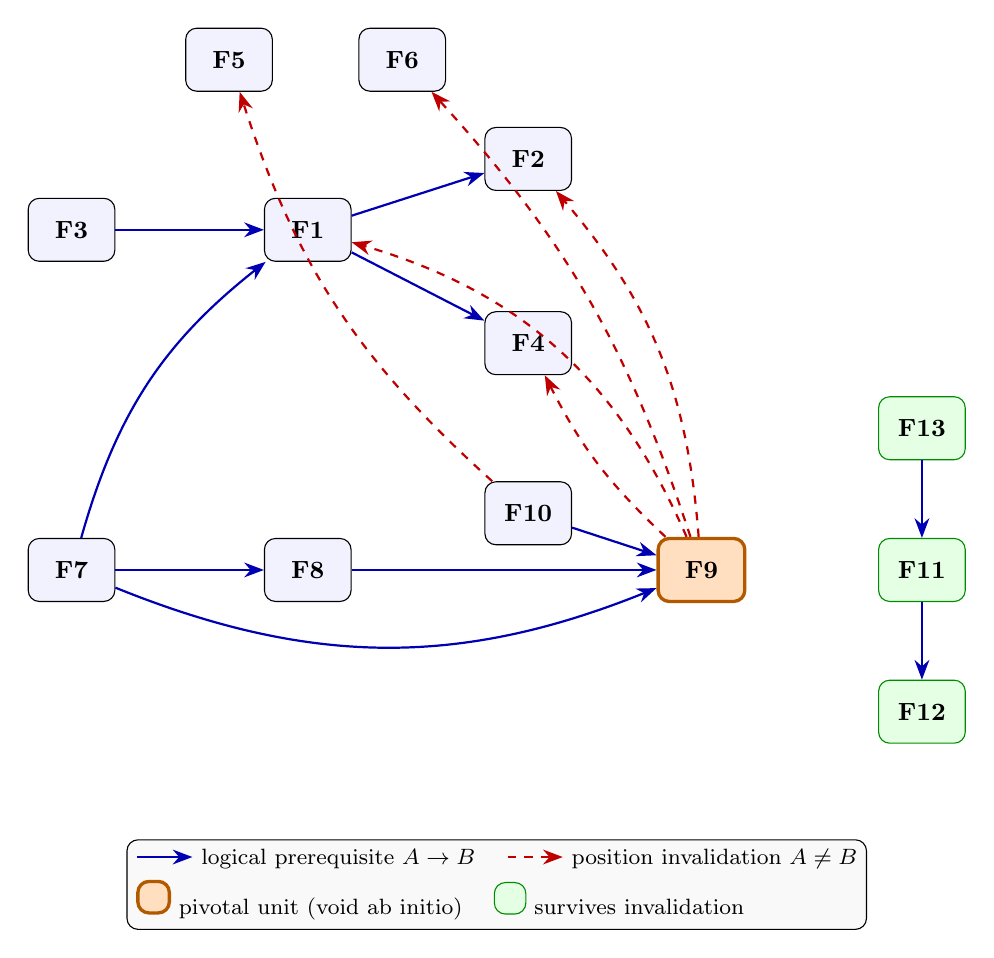
\begin{tikzpicture}[
    >={Stealth[length=2.5mm]},
    x=20mm, y=18mm,
    unit/.style={draw,rounded corners,minimum width=11mm,minimum height=8mm,
                 inner sep=1pt,font=\small\bfseries,fill=blue!5},
    pivot/.style={unit,fill=orange!25,draw=orange!70!black,very thick},
    survive/.style={unit,fill=green!10,draw=green!55!black},
    prereq/.style={->,blue!70!black,thick},
    invalid/.style={->,red!75!black,dashed,thick},
  ]

  % Nodes placed on an explicit (col,row) grid so none overlap.
  % Distinct columns: F2/F4 sit at col 2.9; F9/F10 at col 4.0; UE at col 5.4.
  % Distinct rows keep the F4 / F10 stack well separated.

  % --- defendant's argument (top row) ---
  \node[unit] (f5) at (1.0,3.6) {F5};
  \node[unit] (f6) at (2.1,3.6) {F6};

  % --- breach-of-contract cluster ---
  \node[unit] (f3) at (0,2.4)   {F3};
  \node[unit] (f1) at (1.5,2.4) {F1};
  \node[unit] (f2) at (2.9,2.9) {F2};
  \node[unit] (f4) at (2.9,1.6) {F4};

  % --- agreement / fraud cluster (bottom) ---
  \node[unit]  (f7)  at (0,0)    {F7};
  \node[unit]  (f8)  at (1.5,0)  {F8};
  \node[unit]  (f10) at (2.9,0.4) {F10};
  \node[pivot] (f9)  at (4.0,0)  {F9};

  % --- unjust-enrichment cluster (right, survives) ---
  \node[survive] (f13) at (5.4,1.0)  {F13};
  \node[survive] (f11) at (5.4,0)    {F11};
  \node[survive] (f12) at (5.4,-1.0) {F12};

  % --- logical prerequisites ---
  \draw[prereq] (f3) -- (f1);
  \draw[prereq] (f1) -- (f2);
  \draw[prereq] (f1) -- (f4);
  \draw[prereq] (f7) to[bend left=18] (f1);
  \draw[prereq] (f7) -- (f8);
  \draw[prereq] (f7) to[bend right=22] (f9);
  \draw[prereq] (f8) -- (f9);
  \draw[prereq] (f10) -- (f9);
  \draw[prereq] (f13) -- (f11);
  \draw[prereq] (f11) -- (f12);

  % --- position invalidations (from F9 / F10) ---
  \draw[invalid] (f9) to[bend right=25] (f1);
  \draw[invalid] (f9) to[bend right=18] (f2);
  \draw[invalid] (f9) to[bend left=10]  (f4);
  \draw[invalid] (f9) to[bend right=12] (f6);
  \draw[invalid] (f10) to[bend left=15] (f5);

  % --- legend (below the figure, full width) ---
  \node[draw,fill=gray!5,rounded corners,anchor=north,align=left,
        font=\footnotesize] at (2.7,-1.9) {
    \tikz\draw[prereq](0,0)--(7mm,0);~logical prerequisite $A\rightarrow B$
    \quad
    \tikz\draw[invalid](0,0)--(7mm,0);~position invalidation $A\neq B$\\[3pt]
    \tikz\node[pivot,minimum width=4mm,minimum height=4mm]{};~pivotal unit (void ab initio)
    \quad
    \tikz\node[survive,minimum width=4mm,minimum height=4mm]{};~survives invalidation
  };

\end{tikzpicture}
\end{center}

\end{document}
